\documentclass[twocolumn,a4paper,superscriptaddress,preprintnumbers,showpacs,nofootinbib]{revtex4-1}
%\documentclass[prl,twocolumn,a4paper,superscriptaddress,preprintnumbers,showpacs,nofootinbib]{revtex4-1}
%nobibnotes,linenumbers

\usepackage{amsmath}
\usepackage{graphicx}

\def\d{{\rm d}}
\def\un#1{\,{\rm #1}}
\def\ung#1{\quad[{\rm #1}]}
\def\unt#1{[{\rm #1}]}
\def\e{{\rm e}}
\def\etal{et al.}

\setbox123\hbox{$0$}
\setbox124\hbox{$.$}
\def\S{\hbox to\wd123{\hss}}
\def\.{\hbox to\wd124{\hss}}

\def\thanksInst#1{\unskip\footnotemark[#1]}

\bgroup
\catcode`\@=11

\gdef\thanksRef#1#2{%
    \protected@xdef\@thanks{\@thanks\protect\footnotetext[#1]{#2}}%
}
\egroup

\def\hang{\hangindent=\parindent}
\catcode`\>=11
\newskip\itskip \itskip2mm
\newskip\iitskip \iitskip0mm
\newdimen\itindent \itindent3mm
\newdimen\iitindent \iitindent5mm
\def\>{\par\vskip\itskip\parindent\itindent\indent\hang\llap{\hbox to3mm{$\bullet$\hss}}}
\def\>E{\par\vskip\itskip\parindent\itindent\indent\hang\llap{\hbox to3mm{\hss}}}
\def\>>{\par\vskip\iitskip\parindent\iitindent\indent\hang\llap{\hbox to\iitindent{\hss--\ }}}

\def\Name#1{\textsc{#1}, }
\def\REVIEW#1#2#3#4{{\it #1} {\bf #2} (#3) #4}

%----------------------------------------------------------------------------------------------------

\begin{document}

\title{Evidence for non-exponential elastic differential cross-section at low $|\hbox{t}|$ and $\sqrt{\hbox{s}}$ = 8 TeV} % with TOTEM ?

\date{\today}

\collaboration{The TOTEM Collaboration}
\noaffiliation

\input authorlist_prl


\begin{abstract}
Analysis of a new dataset obtained at $\sqrt{s} = 8\un{TeV}$ and $\beta^* = 90\un{m}$ optics.
High statistics (more than $7\cdot10^{6}$ elastic events)
$\Rightarrow$ strongly reduced statistical and systematic uncertainties (each below $1\un{\%}$) % excluding normalisation unc.
$\Rightarrow$ purely exponential behaviour of differential cross-section excluded at more than $7\un{\sigma}$ significance
$\Rightarrow$ new determination of the total cross-section (non-exponential extrapolation), TODO: values, but still compatible
with the previous TOTEM measurements.
THIS IS JUST PLACEHOLDER -----------\\
\vskip2cm
----------- END OF THE PLACEHOLDER
\end{abstract}


\pacs{13.60.Hb}%{Total and inclusive cross sections (including deep-inelastic processes)}

\preprint{CERN-PH-EP-2014-XXX}

\maketitle

%----------------------------------------------------------------------------------------------------
\section{Introduction}

\> new: high-statistics data sample (same fill as DS2 from \cite{prl111}).
\>> eventually beyond dip/bumb
\>> for the moment only what is relevant for extrapolations to $t=0$

SOMEWHERE: x = horizontal, y = vertical

THIS IS JUST PLACEHOLDER -----------\\
\vskip4cm
----------- END OF THE PLACEHOLDER

%----------------------------------------------------------------------------------------------------
\section{Experimental apparatus}

While the full TOTEM apparatus is described elsewhere \cite{totem-jinst}, here only the sub-detector
relevant for elastic scattering measurement is outlined. The Roman Pots (RPs) are movable beam pipe
insertions that approach the LHC beam very closely in order to detect particles scattered to very 
small angles. They are organised in two stations, one on the left (sector 45), one on the right
(sector 56) side of the interaction point (IP). Each station is formed by two units: near ($214\un{m}$
from the IP) and far ($220\un{m}$). Each unit consists of three RPs: one approaching the beam from top,
one from bottom and one horizontally. Since elastic scattering events contain two anti-parallel protons,
the detected events can have two topologies, called diagonals: 45 bottom -- 56 top and 45 top -- 56 bottom.


%----------------------------------------------------------------------------------------------------
\section{Data taking}

The presented measurement is based on data taken in July 2012, during the LHC fill number 2836, where the vertical
RPs were inserted at $9.5\,\sigma_{\rm beam}$. Two (in the beginning) or three (later) bunches were used, with
a typical population of $8\cdot10^{10}$ protons, yielding instantaneous luminosity of about $10^{28}\un{cm^{-2}s^{-1}}$ per bunch. The special
$\beta^* = 90\un{m}$ optics was used... TODO: some description or reference. The main trigger required coincidence between RPs in both arms,
however combining the near and far units of a station in OR for safe efficiency. In the about $11\un{h}$ long
data-taking, a luminosity of $735\un{\mu b^{-1}}$ was accumulated, giving
$7.2\cdot 10^6$ tagged elastic events.

%minimal $|t| = 0.027\un{GeV^2}$ % left edge of left most bin


%----------------------------------------------------------------------------------------------------
\section{Analysis}

The analysis method is very similar to the previously published ones \cite{prl111,epl101-el}. Each diagonal is analysed
separately, some steps are performed independently for each bunch. In this analysis, a different normalisation
approach is used, consequently making all $t$-independent scaling factors (e.g.~inefficiency corrections)
irrelevant.

%--------------------------------------------------
\subsection{Event reconstruction}

\iffalse
\begin{equation}
\label{eq:t}
t = p^2 ({\theta_x^*}^2 + {\theta_y^*}^2)
\end{equation}
TODO: projections of scattering angle
\fi

The horizontal ($\theta_x^*$) and vertical ($\theta_y^*$) projections of the scattering angle and the horizontal
vertex position $x^*$ are reconstructed in each arm from aligned hit positions (e.g.~$x^{\rm N}$ represents horizontal
position of the hit in the near RP):
\begin{equation}
\label{eq:kin 1a}
	\begin{aligned}
		\theta_x^* &= {v_x^{\rm N} x^{\rm F} - v_x^{\rm F} x^{\rm N}\over v_x^{\rm N} L_x^{\rm F} - v_x^{\rm F} L_x^{\rm N}}\ ,\qquad
		\theta_y^* = {1\over 2} \left( {y^{\rm N}\over L_y^{\rm N}} + {y^{\rm F}\over L_y^{\rm F}} \right)\ ,\\
		x^* &= {L_x^{\rm N} x^{\rm F} - L_x^{\rm F} x^{\rm N}\over L_x^{\rm N} v_x^{\rm F} - L_x^{\rm F} v_x^{\rm N}}\ , \\
	\end{aligned}
\end{equation}
where $L$'s stand for effective length and $v$'s for magnification optical functions. These formulae minimise the
impact of optics imperfections and, in the horizontal projection, decouple the scattering angle and vertex terms.
While the one-arm reconstruction is essential for elastic event tagging, using both arms
\begin{equation}
\label{eq:kin 2a}
\theta_x^* = (\theta_x^{*L} + \theta_x^{*R})/2\ ,\quad \theta_y^* = (\theta_y^{*L} + \theta_y^{*R})/2\ .
\end{equation}
leads to resolution improvement for already tagged events.

{\bf Alignment}. The standard three-step procedure \cite{totem-ijmp} has been applied, reducing the uncertainty to $2\un{\mu m}$ (horizontal shifts), $100\un{\mu m}$ (vertical shifts) and rotations $0.2\un{mrad}$ for each unit (common for top and bottom RPs). Propagated to the scattering angles, the shifts lead to uncertainties %(double-arm)
$0.8\un{\mu rad}$ (horizontal) and $0.2\un{\mu rad}$ (vertical).
%(effect disappears when diagonals combined)
% rotation th_x^reco = th_x^true + A * th_y, si[A] = 0.02

{\bf Optics}. The optics matching method \cite{totem-optics} has been applied. The residual uncertainty has a form of factors scaling the scattering angles: % double-arm; before matching $0.48\un{\%}$ (hor), $0.90\un{\%}$
$0.21\un{\%}$ (horizontal) and $0.25\un{\%}$ (vertical), including the effects of magnet harmonics.

{\bf Resolution} Statistical fluctuations in the reconstructed scattering angles occur due to the beam divergence and, in horizontal projection, also detector resolution. Good description of these effects is essential for several corrections discussed below. The angular resolution is studied through differences $\theta_{x,y}^{*R} - \theta_{x,y}^{*L}$. Since in good approximation the fluctuations are independent in each arm, the distribution of the difference is just twice wider than the fluctuation of angles in Eq.~(\ref{eq:kin 2a}). Generally, the distributions are well Gaussian, the small non-Gaussianity is decreasing with time. The resolutions were found to deteriorate by $0.1$ to $0.2\un{\mu rad}$ during the run, the typical values in the beginning were $1.6\un{\mu rad}$ (vertical) and $4.5\un{\mu rad}$ (horizontal -- moreover diagonal dependent).
\iffalse
The resolution in $\theta_y^*$ decreased from $1.6$ to $1.7\un{\mu rad}$ from the beginning to the end of the fill (DS3+DS4), for $\theta_x^*$ from $4.6$ to $4.8\un{\mu rad}$ (45b -- 56t) and from $4.3$ to $4.4\un{\mu rad}$ (45t -- 56b). In fact, just means over all bunches -- in analysis bunches treated independently. Comparing x and y, the contribution from the RP spatial resolution is evident. A cross check, horizontal beam div. from vertex distribution (sigma 145 to 185 urad, diagonal independent) % 2.3 to 2.9 urad
, the sensor contribution (2-arm) is $4.3$ (45b) and $4.0$ urad (45t), time independent. With the same method, not only RMS, but also shape. Generally, gaussian-like, with non-gaussianity decreasing with time. Non-gaussianinty taken accounted in systematic uncertainties. The original assumption of identical resolutions in both arms can be verified by checking the beam emittances. They give beam divergences compatible with our observations and indicate that a possible left-right imbalance could be of order $15\un{\%}$, which is used for uncertainty estimation.
\fi

%--------------------------------------------------
\subsection{Differential cross-section}

For a given $t$ bin, the value of differential cross-section is evaluated by selecting and counting elastic events as follows
\begin{equation}
{\d\sigma\over \d t}(\hbox{bin}) =
	{\cal N}\, {\cal U}({\rm bin})\, {\cal B}\ 
	{\sum\limits_{t \in \hbox{bin}} {\cal A}(\theta_x^*, \theta_y^*)\, {\cal E}(\theta_y^*)\over \Delta t}\ ,
\end{equation}
where $\Delta t$ is the width of the bin, ${\cal N}$ is a normalisation factor and the other symbols stand for various correction factors:
 ${\cal U}$ for unfolding, ${\cal B}$ for background subtraction, ${\cal A}$ for acceptance correction and ${\cal E}$ for detection and reconstruction efficiency.

{\bf Tagging}. The cuts used to select the elastic events are summarized in Tab.~\ref{tab:cuts}, all are applied at $4\sigma$-level. Cuts 1 and 2 require the reconstructed-track collinearity between the left and right arm. Cut 5 ensures that the protons come from the same vertex (horizontally). Cuts 3 and 4 control the elasticity -- if proton loses momentum, the vertical position-angular correlation at RPs is lost. The tagging efficiency is studied by applying the cuts also at $5\un{\sigma}$-level. This selection yields $0.5\un{\%}$ more events, uniformly in $|t|$ -- thus the inefficiency is irrelevant for this analysis.

\begin{table}
\caption{The elastic selection cuts. The superscripts R and L refer to the right and left arm, the N and F corresponds to the near and far units. The constant $\alpha = L_y^{\rm F} / L_y^{\rm N} - 1 \approx 0.107$. The right-most column gives a typical RMS of the cut distribution.
}
\label{tab:cuts}
\begin{center}
\vskip-3mm
\begin{tabular}{ccc}\hline\hline
number & cut & RMS ($\equiv 1\sigma$)\cr\hline
1 & $\theta_x^{*\rm R} - \theta_x^{*\rm L}$				& $9.5\un{\mu rad}$	\cr
2 & $\theta_y^{*\rm R} - \theta_y^{*\rm L}$				& $3.3\un{\mu rad}$	\cr
3 & $\alpha\,y^{\rm R,N} - (y^{\rm R,F} - y^{\rm R,N})$	& $18\un{\mu m}$	\cr
4 & $\alpha\,y^{\rm L,N} - (y^{\rm L,F} - y^{\rm L,N})$	& $18\un{\mu m}$	\cr
5 & $x^{*\rm R} - x^{*\rm L}$							& $8.5\un{\mu m}$ 	\cr\hline\hline
\end{tabular}
\end{center}
\end{table}

{\bf Background}. Studying distributions of discriminators from Tab.~\ref{tab:cuts} under various cut combinations allows for separation of signal and background contributions. Then, the background component can be interpolated from background region ($> 4\un{\sigma}$) to the signal region ($< 4\un{\sigma}$), yielding an background/signal estimate of $10^{-4}$.
% (for th x, th y and vtx x cuts). ${\cal B} = 1$, anyway irrelevant due to the normalisation approach.

{\bf Acceptance correction} ${\cal A}$. Two detection limitations have been identified: detector coverage (mostly the edge facing beam, relevant for small $|\theta_y^*|$) and LHC apertures (high $|\theta_y^*|$). An event can fall outside acceptance due to azimuthal angle $\phi^*$ or due to fluctuations if near the acceptance boundaries. For the former, the expected azimuthal symmetry is verified for the data within the acceptance and then applied outside -- the correction factor is given by the ratio of $\theta^*$-constant arc(s) inside acceptance to the full circle. The latter effect can be corrected as the fluctuations are well described (see above). For the uncertainties, the error of the distribution width and shape as well as left-right imbalance (${\cal O}(15\un{\%})$ from emittance measurements) have been considered.
% non-gauss, imbalance both few per-mille within final data

\iffalse
\begin{equation}
\label{acceptance}
{\cal A_{\rm sm}}(\theta_y^*)^{-1} = {1\over 2} \left(
	\mathop{\rm Erf} {\min(\theta_y^{*,R,max} - |\theta_y^*|, |\theta_y^*| - \theta_y^{*,L,min})\over \sigma^{1a}_{\theta_y^*}}
	- \mathop{\rm Erf} {\max(\theta_y^{*,R,min} - |\theta_y^*|, |\theta_y^*| - \theta_y^{*,L,max})\over \sigma^{1a}_{\theta_y^*}}
\right)
\end{equation}

\begin{equation}
\label{acceptance}
{\cal A_{\phi}}(\theta_y^*) = {
	2\pi\over 
	\hbox{arc length with $\theta_y^*$ between } \max(\theta_y^{*,L,min}, \theta_y^{*,R,min}) \hbox{ and } \min(\theta_y^{*,L,max}, \theta_y^{*,R,max})
}
\end{equation}
\fi

{\bf Efficiency corrections} include corrections for inefficiencies from various sources: trigger inefficiency ${\cal I}_{\rm trig}$, reconsctruction inefficiency ${\cal I}_{\rm det}$ and pile-up inefficiency ${\cal I}_{\rm PU}$ (RPs unable to resolve multiple tracks):

\begin{equation}
\label{efficiency}
	\begin{aligned}
		{\cal E}(\theta_y^*) &= {1\over 1 - {\cal I}_{\rm trig}} {1\over 1 - {\cal I}_{\rm det}(\theta_y^*)} {1\over 1 - {\cal I}_{\rm PU}}\ ,\\
		{\cal I}_{\rm det}(\theta_y^*) &= \sum\limits_{i\in \rm RPs} {\cal I}^i_{3/4}(\theta_y^*) + 2 {\cal I}_{2/4}\\
	\end{aligned}
\end{equation}

The trigger and pile-up inefficiencies are mentioned for completeness only, since they do not affect the distribution shape, their values are not relevant the presented analysis due to a different way of final normalisation. The efects were nevertheless studied with techniques used in previous publications yielding expectable results.

Detector efficiency. Standard technique: 3/4 for every RP (${\cal I} \approx 1\un{\%}$ near and $2.5\un{\%}$ far) and 2/4 (${\cal I} = 1.5\un{\%}$) for the nears. 3/4 studied as function of $\theta_y^*$ to disentangle efficiency from acceptance effects. Furthermore, due to high statistics, gentle efficiency decrease with increasing $|\theta_y^*|$ was observed and taken into account. Average slope of the decrease per RP was $80\un{rad^{-1}}$ with a typical uncertainty of $8\un{rad^{-1}}$ for DS4.

%Trigger efficiency. Zero-bias data stream, events tagged as elastic, look at the trigger flag. NOT IN DS4 !!!
%For example for DS2, at $95\un{\%}$ CL, ${\cal I}_{\rm trig} < 8\cdot10^{-4}$. Anyway irrelevant.

{\bf Unsmearing}. Apriory: small effect due to the good angular resolution (above). 2 iterations: fit, Monte-Carlo calculation of the effect, correction of the ds/dt. Correction $|1 - {\cal U}| < 3\un{\%}$

{\bf Normalisation}. TODO: ${\cal N}$, same integral between $|t| = 0.027$ and $0.083\un{GeV^2}$ wrt.~dataset 1 from \cite{prl111}. Leading uncertainty: lumi error from DS2 ($4.2\un{\%}$), transfer to DS4 negligible (few per-mille)

{\bf Binning} Two binnings used. ``Optimised'': bin size = one smearing sigma. ``Per-mille'': each bin gets about one per-mille of the events.

{\bf TODO: Estimate of systematics} Only the general approach. MC and num.~int. techniques for propagation 

%--------------------------------------------------
\subsection{Final data merging}

\> central values - per bin: weighted mean, weight = $1/\sigma^2(stat)$

\> statistical uncertainties - propagated as for central values, but for optimised binning:
\>> too good fits, too little point-to-point fluctuation
\>> test: divide data into sub-samples, same analysis, then calculate fluctuations in all bins $\Rightarrow$ same conclusion
\>> not in per-mille binning
\>> interpretation -- TODO
\>> solution, data in optimised binning: uncertainties scaled by $1/1.17596$ to give the same normalised $\chi^2$ as for per-mill binning

\> systematics
\>> combine systematics from each diagonal, take into account the correlations -- e.g. vertical shifts
\>> list of leading uncertainties: optics modes 1 and 2, beam momentum -- link to Tab.~\ref{tab:data}
\>> recipe to build covariance matrix

%----------------------------------------------------------------------------------------------------
\section{Results}

% --- the results drawn from the optimised binning

The final differential cross-section in the optimised binning is presented in Tab.~\ref{tab:data}. Since it exhibits an exponential-like fall off, for visualisation purposes, it is preferable to plot the relative of the cross-section from a reference exponential% subtracting the main component
, see Fig.~\ref{fig:data rel ob}. This plot immediately suggests non-exponentiality of the data. To quantify this observation, a series of fits has been made using this parametrisation:
\begin{equation}
\label{fit param}
{\d\sigma\over\d t}(t) = \left. \d\sigma\over\d t\right|_{0} \ \exp\left( \sum\limits_{i = 1}^{N_{b}} b_i\, t^i \right)
\end{equation}
The fits have been performed by minimising standard $\chi^2$ with covariance matrix given by the sum of the statistical and systematic components. The fit results are shown in Fig.~\ref{fig:data rel ob}, clearly indicating that the purely-exponential fit ($N_b = 1$) is excluded at $7.2\un{\sigma}$ significance. The other two fits present very reasonable p-values and can, therefore, be used for total cross-section estimation
\begin{equation}
\label{eq:si tot}
\sigma_{\rm tot}^2 = {16\pi\, (\hbar c)^2\over 1 + \rho^2}\, \left. \d\sigma_{\rm el}\over\d t\right|_0\ ,
\end{equation}
for the first time using non-exponential extrapolation to $t=0$. Using the COMPETE \cite{compete} preferred-model extrapolation of $\rho = 0.140\pm 0.007$ yields
\begin{equation}
\label{eq:si tot results}
	\begin{aligned}
		N_b &= 2:\quad \sigma_{\rm tot} = (100.8 \pm 2.1)\un{mb}\ ,\\	% A = 529.3 +- 21.9
		N_b &= 3:\quad \sigma_{\rm tot} = (101.2 \pm 2.1)\un{mb}\ .\\	% A = 533.5 +- 21.9
	\end{aligned}
\end{equation}
which are well compatible with our previous measurement using the luminosity-independent method \cite{prl111}.


% --- results from per-mille binning

The incompatibility between pure exponential behaviour and the data with the per-mille binning can be shown equally well. However, since the number of points is drastically increased, the $\chi^2$ test does not have sufficient sensitivity and a different test is used. Assume that the data can be described by a pure exponential, then the fit parameters shall have compatible values for fits over different regions. Such fits are shown in Fig.~\ref{fig:data rel cpb0.001}, for regions below and above $|t| = 0.07\un{GeV^2}$. Although the overall fit quality is satisfactory, the difference in fit parameters excludes their compatibility at $7.7\un{\sigma}$. This, in turn, rules out the hypothesis of purely exponential behaviour of the data.

\iffalse
	split details
                A = 529.299 +- 21.951
                B1 = -19.678 +- 0.074
                B2 = 514.681 +- 21.953
                B3 = -19.264 +- 0.057

 A1 − A2 = 14.617 ± 1.789 ⇒ 8.2 σ
 B1 − B2 = −0.414 ± 0.056 ⇒ 7.4 σ
\fi




\begin{table*}
\vskip-5mm
\caption{%
The elastic differential cross-section as determined in this analysis using the optimised binning. The left-most three columns describe bins in $t$. The representative point give the $t$ value suitable for fitting \cite{lafferty94}. %uncertainty due to different fit models negligible:$10^{-7}\un{GeV^2}$
The other columns are related to the differential cross-section. The right-most four columns give the leading systematic uncertainty modes (see above TODO). TODO: optimise number of digits, spacing.
}
\vskip-3mm
\label{tab:data}
\begin{center}
\scriptsize
\setlength{\tabcolsep}{3.5pt}
\begin{tabular}{ccc@{\hskip15pt}ccccccc}
\hline
\hline
\multispan3\hss $|t|$ bin $\unt{GeV^2}$\hss & \multispan7\hss $\d\sigma/\d t \ung{mb/GeV^2}$ \hss \cr
left & right & repres. & value & stat.     & full syst. & norm. & optics   & optics   & beam\cr
edge & edge  & point   &       & unc.      & unc.       &       & mode 1   & mode 2   & momentum\cr
\hline
$0.027$ & $0.030$ & $0.029$ & $300.945$ & $0.612$ & $12.909$ & $12.890$ & $-0.473$ & $-0.260$ & $+0.254$ \cr
$0.030$ & $0.033$ & $0.032$ & $284.042$ & $0.554$ & $12.130$ & $12.113$ & $-0.495$ & $-0.214$ & $+0.204$ \cr
$0.033$ & $0.037$ & $0.035$ & $265.588$ & $0.506$ & $11.370$ & $11.355$ & $-0.484$ & $-0.172$ & $+0.157$ \cr
$0.037$ & $0.040$ & $0.038$ & $247.896$ & $0.465$ & $10.632$ & $10.618$ & $-0.472$ & $-0.133$ & $+0.114$ \cr
$0.040$ & $0.044$ & $0.042$ & $231.953$ & $0.430$ & $ 9.917$ & $ 9.904$ & $-0.459$ & $-0.097$ & $+0.074$ \cr
$0.044$ & $0.047$ & $0.046$ & $215.353$ & $0.398$ & $ 9.225$ & $ 9.213$ & $-0.446$ & $-0.064$ & $+0.038$ \cr
$0.047$ & $0.051$ & $0.049$ & $199.885$ & $0.369$ & $ 8.559$ & $ 8.546$ & $-0.431$ & $-0.034$ & $+0.005$ \cr
$0.051$ & $0.055$ & $0.053$ & $184.554$ & $0.342$ & $ 7.917$ & $ 7.905$ & $-0.416$ & $-0.007$ & $-0.024$ \cr
$0.055$ & $0.060$ & $0.057$ & $170.715$ & $0.318$ & $ 7.303$ & $ 7.290$ & $-0.400$ & $+0.017$ & $-0.050$ \cr
$0.060$ & $0.064$ & $0.062$ & $156.615$ & $0.295$ & $ 6.715$ & $ 6.703$ & $-0.383$ & $+0.038$ & $-0.072$ \cr
$0.064$ & $0.068$ & $0.066$ & $142.958$ & $0.274$ & $ 6.155$ & $ 6.142$ & $-0.366$ & $+0.056$ & $-0.091$ \cr
$0.068$ & $0.073$ & $0.071$ & $131.310$ & $0.254$ & $ 5.623$ & $ 5.610$ & $-0.348$ & $+0.072$ & $-0.107$ \cr
$0.073$ & $0.078$ & $0.076$ & $119.589$ & $0.236$ & $ 5.120$ & $ 5.106$ & $-0.330$ & $+0.084$ & $-0.120$ \cr
$0.078$ & $0.083$ & $0.081$ & $108.278$ & $0.218$ & $ 4.645$ & $ 4.631$ & $-0.312$ & $+0.095$ & $-0.131$ \cr
$0.083$ & $0.089$ & $0.086$ & $ 97.732$ & $0.202$ & $ 4.199$ & $ 4.184$ & $-0.294$ & $+0.102$ & $-0.138$ \cr
$0.089$ & $0.094$ & $0.091$ & $ 87.916$ & $0.186$ & $ 3.781$ & $ 3.766$ & $-0.275$ & $+0.108$ & $-0.143$ \cr
$0.094$ & $0.100$ & $0.097$ & $ 78.866$ & $0.172$ & $ 3.391$ & $ 3.376$ & $-0.257$ & $+0.112$ & $-0.146$ \cr
$0.100$ & $0.106$ & $0.103$ & $ 70.641$ & $0.158$ & $ 3.029$ & $ 3.014$ & $-0.239$ & $+0.114$ & $-0.146$ \cr
$0.106$ & $0.112$ & $0.109$ & $ 62.480$ & $0.145$ & $ 2.694$ & $ 2.678$ & $-0.221$ & $+0.114$ & $-0.145$ \cr
$0.112$ & $0.119$ & $0.115$ & $ 55.454$ & $0.133$ & $ 2.386$ & $ 2.369$ & $-0.204$ & $+0.112$ & $-0.142$ \cr
$0.119$ & $0.125$ & $0.122$ & $ 48.733$ & $0.122$ & $ 2.103$ & $ 2.086$ & $-0.187$ & $+0.110$ & $-0.138$ \cr
$0.125$ & $0.132$ & $0.129$ & $ 42.712$ & $0.111$ & $ 1.844$ & $ 1.828$ & $-0.171$ & $+0.106$ & $-0.132$ \cr
$0.132$ & $0.140$ & $0.136$ & $ 37.277$ & $0.102$ & $ 1.610$ & $ 1.594$ & $-0.155$ & $+0.101$ & $-0.126$ \cr
$0.140$ & $0.147$ & $0.143$ & $ 32.207$ & $0.092$ & $ 1.398$ & $ 1.382$ & $-0.140$ & $+0.096$ & $-0.119$ \cr
$0.147$ & $0.155$ & $0.151$ & $ 27.731$ & $0.084$ & $ 1.207$ & $ 1.191$ & $-0.126$ & $+0.091$ & $-0.111$ \cr
$0.155$ & $0.163$ & $0.159$ & $ 23.827$ & $0.076$ & $ 1.035$ & $ 1.021$ & $-0.094$ & $+0.086$ & $-0.102$ \cr
$0.163$ & $0.172$ & $0.168$ & $ 20.364$ & $0.072$ & $ 0.881$ & $ 0.870$ & $-0.058$ & $+0.079$ & $-0.094$ \cr
$0.172$ & $0.181$ & $0.176$ & $ 17.249$ & $0.067$ & $ 0.746$ & $ 0.736$ & $-0.030$ & $+0.073$ & $-0.085$ \cr
$0.181$ & $0.190$ & $0.185$ & $ 14.480$ & $0.063$ & $ 0.628$ & $ 0.619$ & $-0.008$ & $+0.066$ & $-0.077$ \cr
$0.190$ & $0.200$ & $0.195$ & $ 12.124$ & $0.059$ & $ 0.526$ & $ 0.517$ & $+0.005$ & $+0.060$ & $-0.069$ \cr
\hline
\hline
\end{tabular}
\end{center}
\vskip-10mm
\end{table*}

\begin{figure*}
\vskip-5mm
\begin{center}
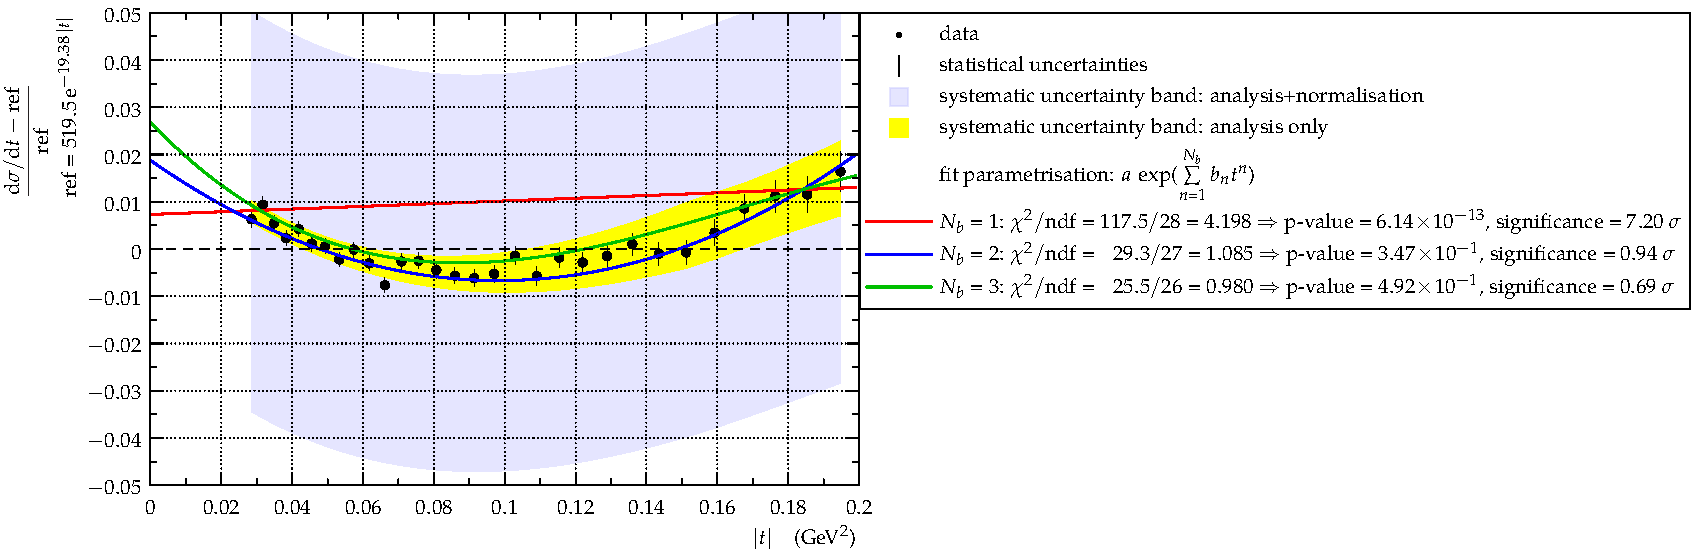
\includegraphics[height=6.5cm]{fig/t_dist_rel_with_fits.pdf}
\vskip-6mm
\caption{%
The final differential cross-section using the optimised binning and plotted as relative difference to a reference exponential (see vertical axis). The black dots represent data points with statistical uncertainty bars. The blue band corresponds to full systematic uncertainty, the yellow one shows all systematic contribution except normalisation. The coloured lines correspond to fits with parametrisation Eq.~(\ref{fit param}).
%using full covariance matrix.
TODO: describe fit quality measures?}
\label{fig:data rel ob}
\end{center}
\vskip-2mm
\end{figure*}

\begin{figure*}
%\vskip-10mm
\begin{center}
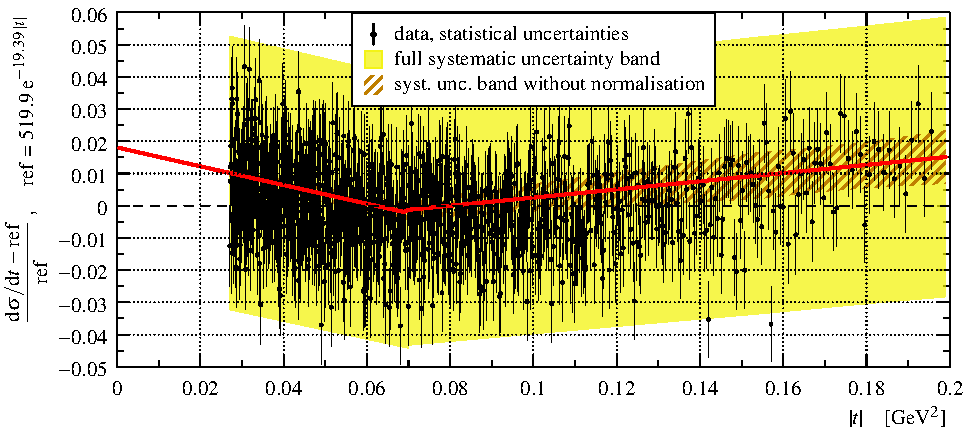
\includegraphics[height=6.5cm]{fig/t_dist_rel_with_split_fit.pdf}
\vskip-6mm
\caption{
The final differential cross-section using the per-mille binning and plotted as relative difference to the reference exponential (see vertical axis). The black dots represent data points with statistical uncertainty bars. The blue band corresponds to full systematic uncertainty, the yellow one shows all systematic contribution except normalisation. The green line shows pure exponential fits in regions below and above $|t| = 0.07\un{GeV^2}$.
}
\label{fig:data rel cpb0.001}
\end{center}
%\vskip-35mm
\end{figure*}


%----------------------------------------------------------------------------------------------------
\section{Discussion/Conclusions/Outlook}

\> will extend this analysis beyond the dip
\> link to the $1000\un{m}$ paper?


%----------------------------------------------------------------------------------------------------

\acknowledgements
THIS IS JUST PLACEHOLDER -----------
We are indebted to the beam optics development team
%({\sc A.~Verdier} in the initial phase, {\sc H.~Burkhardt}, {\sc G.~M\" uller}, {\sc S.~Redaelli}, {\sc J.~Wenninger}, {\sc S.~M.~White})
for the design, the thorough preparations and the successful commissioning of the $\beta^* = 90\un{m}$ optics. We congratulate the CERN accelerator groups for the very smooth operation in 2011. We thank
%{\sc M.~Ferro-Luzzi}
the LHC machine coordinators for scheduling the dedicated fills.

This work was supported by the institutions listed on the front page and partially also by NSF (US), the Magnus
Ehrnrooth foundation (Finland), the Waldemar von Frenckell foundation (Finland), the Academy of
Finland, the OTKA grant NK 101438, 73143 (Hungary) and the NKTH-OTKA grant 74458 (Hungary).
----------- END OF THE PLACEHOLDER


%----------------------------------------------------------------------------------------------------
\begin{thebibliography}{99}

\bibitem{totem-jinst}
    %The TOTEM Experiment at the CERN Large Hadron Collider, JINST 3 S08007, 2008
	\Name{Anelli G.~\etal{}~(TOTEM Collaboration)}
	\REVIEW{JINST}{3}{2008}{S08007}

\bibitem{totem-ijmp}
	\Name{Antchev G.~\etal{}~(TOTEM Collaboration)}
	\REVIEW{Int.~J.~Mod.~Phys.~A}{28}{2013}{1330046}

\bibitem{totem-optics}
	\Name{Antchev G.~\etal{}~(TOTEM Collaboration)}
	LHC Optics Measurement with Proton Tracks Detected by the Roman Pots of the TOTEM Experiment, 
	arXiv:1406.0546

\bibitem{prl111}
	\Name{Antchev G.~\etal{}~(TOTEM Collaboration)}
	\REVIEW{Phys.~Rev.~Lett.}{111}{2013}{012001}

\bibitem{epl101-el}
	\Name{Antchev G.~\etal{}~(TOTEM Collaboration)}
	\REVIEW{Europhys.~Lett.}{101}{2013}{21002}

\bibitem{lafferty94}
 	% Where to stick your data points: The treatment of measurements within wide bins
	\Name{Lafferty G.~D.~and Wyatt T.~R.}
	\REVIEW{Nucl.\ Instrum.\ Meth.}{A 355}{1995}{541}

\bibitem{compete} 
	\Name{Cudell~J.~R.~\etal{} (COMPETE Collaboration)}
	\REVIEW{Phys.\ Rev.\ Lett.}{89}{2002}{201801}


\iffalse

\bibitem{epl95}
    %Proton-proton elastic scattering at the LHC energy of \sqrt{s} = 7 TeV, Europhys. Lett. 95 (2011) 41001,CERN-PH-EP-2011-101 
	\Name{Antchev G.~\etal{}~(TOTEM Collaboration)}
	\REVIEW{Europhys.~Lett.}{95}{2011}{41001}

\bibitem{epl96}
    %First measurements of the total proton-proton cross-section at the LHC energy of $\sqrt s =7\,\rm TeV$ CERN-PH-EP-2011-158
	\Name{Antchev G.~\etal{}~(TOTEM Collaboration)}
	\REVIEW{Europhys.~Lett.}{96}{2011}{21002}

\bibitem{epl101-inel}
	\Name{Antchev G.~\etal{}~(TOTEM Collaboration)}
	\REVIEW{Europhys.~Lett.}{101}{2013}{21003}

\bibitem{epl101-tot}
	\Name{Antchev G.~\etal{}~(TOTEM Collaboration)}
	\REVIEW{Europhys.~Lett.}{101}{2013}{21004}

\bibitem{jan_thesis}
	\Name{Ka\v spar J.}
	PhD Thesis, CERN-THESIS-2011-214, {\tt http://cdsweb.cern.ch/record/1441140}

\bibitem{mario_ipac_2011}
	\Name{Deile M.}
	{\it The First 1 1/2 Years of TOTEM Roman Pot Operation at LHC}, in
	{\it Proceedings of the 2nd International Particle Accelerator Conference (IPAC 2011), San Sebastian, Spain}. 
	%{\tt http://accelconf.web.cern.ch/AccelConf/IPAC2011/papers/mopo011.pdf}
	arXiv:1110.5808v1

%\bibitem{pdg} 
%	\Name{Nakamura K.~\etal{} (Particle Data Group)}
%	\REVIEW{J.~Phys.}{G37}{2010}{075021}

\bibitem{B_vs_s}
	\Name{ISR (CR Collaboration)} \REVIEW{Phys.~Lett.}{B62}{1976}{460}; 
	\Name{ISR (ACHGT Collaboration)} \REVIEW{Phys.~Lett.}{B39}{1972}{663}; 
	\Name{ISR (R-211)} \REVIEW{Nucl.~Phys.}{B262}{1985}{689}; 
	\Name{ISR (R-210)} \REVIEW{Phys.~Lett.}{B115}{1982}{495}; 
	\Name{UA1} \REVIEW{Phys.~Lett.}{B147}{1984}{385}; 
	\Name{UA4} \REVIEW{Phys.~Lett.}{B127}{1983}{472} and \REVIEW{Phys. Lett.}{B198}{1987}{583}; 
	\Name{UA4/2} \REVIEW{Phys.~Lett.}{B316}{1993}{448}; 
	\Name{CDF} \REVIEW{Phys.~Rev.}{D50}{1994}{5518}; 
	\Name{E710} \REVIEW{Phys.~Rev.~Lett.}{68}{1992}{2433} and \REVIEW{Nuovo Cimento}{A106}{1992}{123}; 
	\Name{D0} D0 Note 6056-CONF; 
	\Name{pp2pp} \REVIEW{Phys.~Lett.}{B579}{2004}{245}

\fi

\end{thebibliography}



\end{document}
